%% Substituir o [PENDENTE: Inserir as figuras e tabelas...] por este bloco.
%% As imagens estão em figuras/ (copiar a pasta para o Overleaf).

Os experimentos seguem o desenho $2\times 2$ da Figura~\ref{fig:matriz-experimental}: allowlist ligada ou não, e firmware limpo ou adulterado. A Figura~\ref{fig:tabela-comparacao} e as demais reportam o lote de 30 amostras por célula, com intervalo sequencial entre POSTs. O que o placeholder pedia como ``tempo de assinatura no ESP32'' e ``taxa de sucesso sob carga'' \emph{não foi medido}: a assinatura EVM ocorre no PC do relay, e o lote não é um teste de estresse. Reporta-se, no lugar, o tempo até o envio da transação no relay e a taxa de aceite no lote sequencial.

\begin{figure}[htbp]
\centering
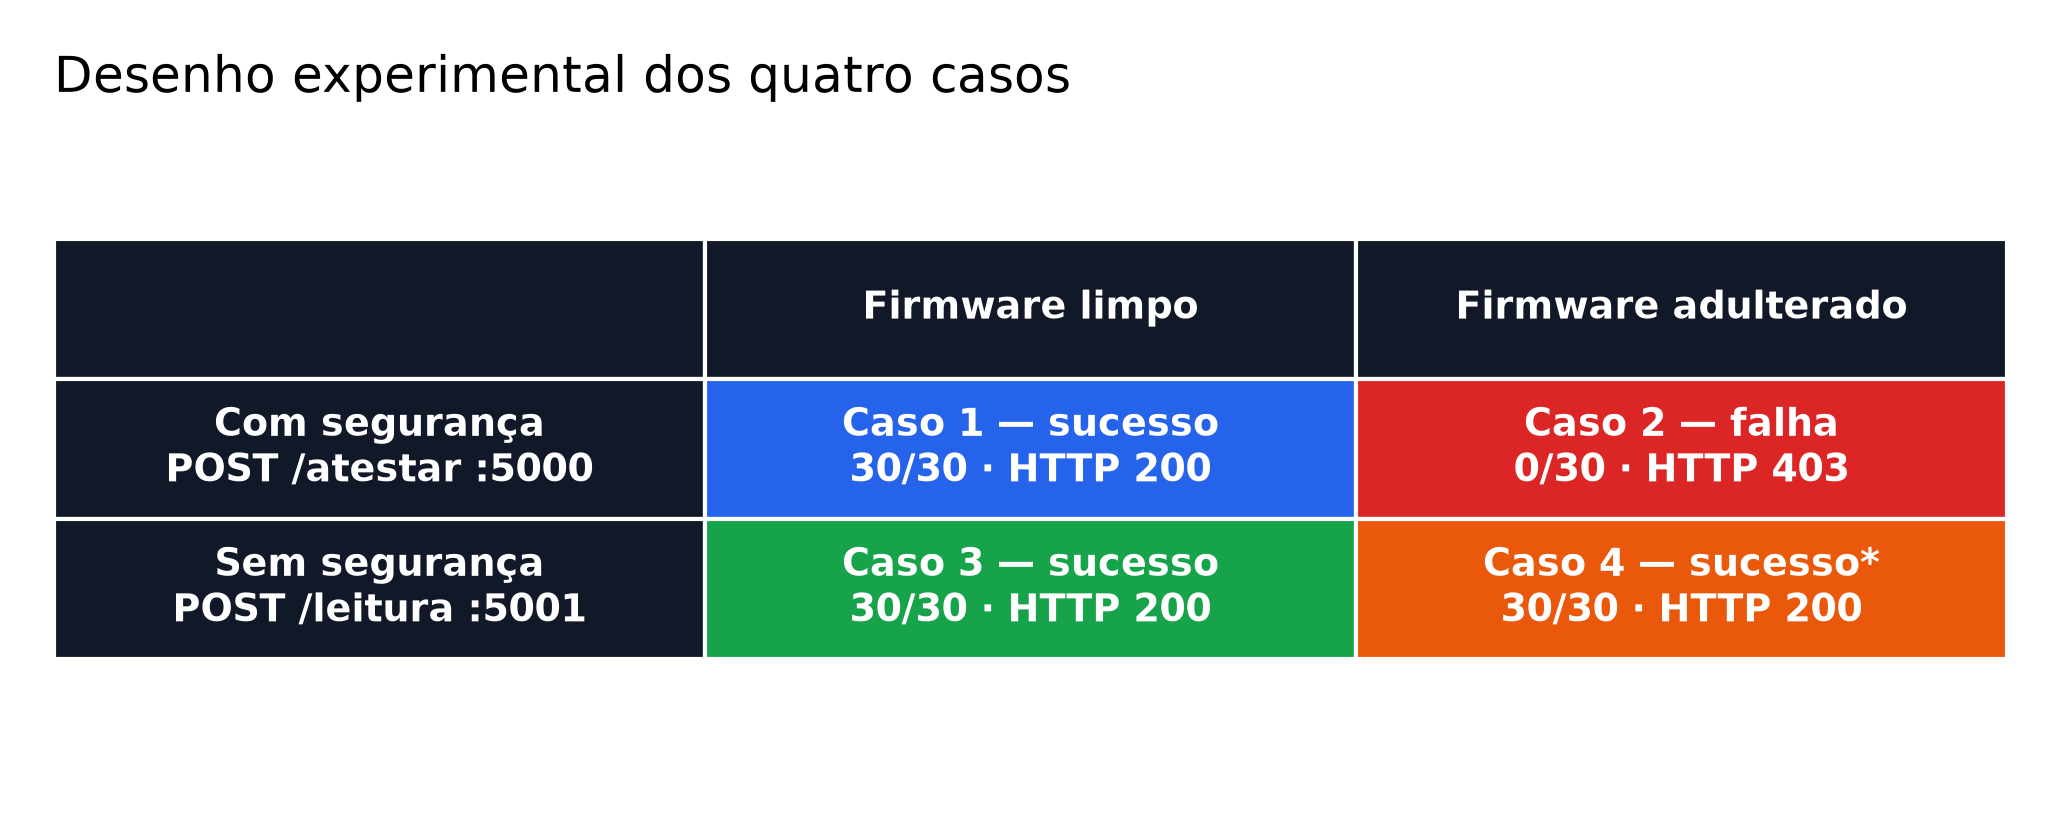
\includegraphics[width=0.92\textwidth]{figuras/matriz-experimental.png}
\caption{Desenho experimental dos quatro tratamentos (allowlist $\times$ adulteração do \texttt{.ino}).}
\label{fig:matriz-experimental}
\end{figure}

\begin{figure}[htbp]
\centering
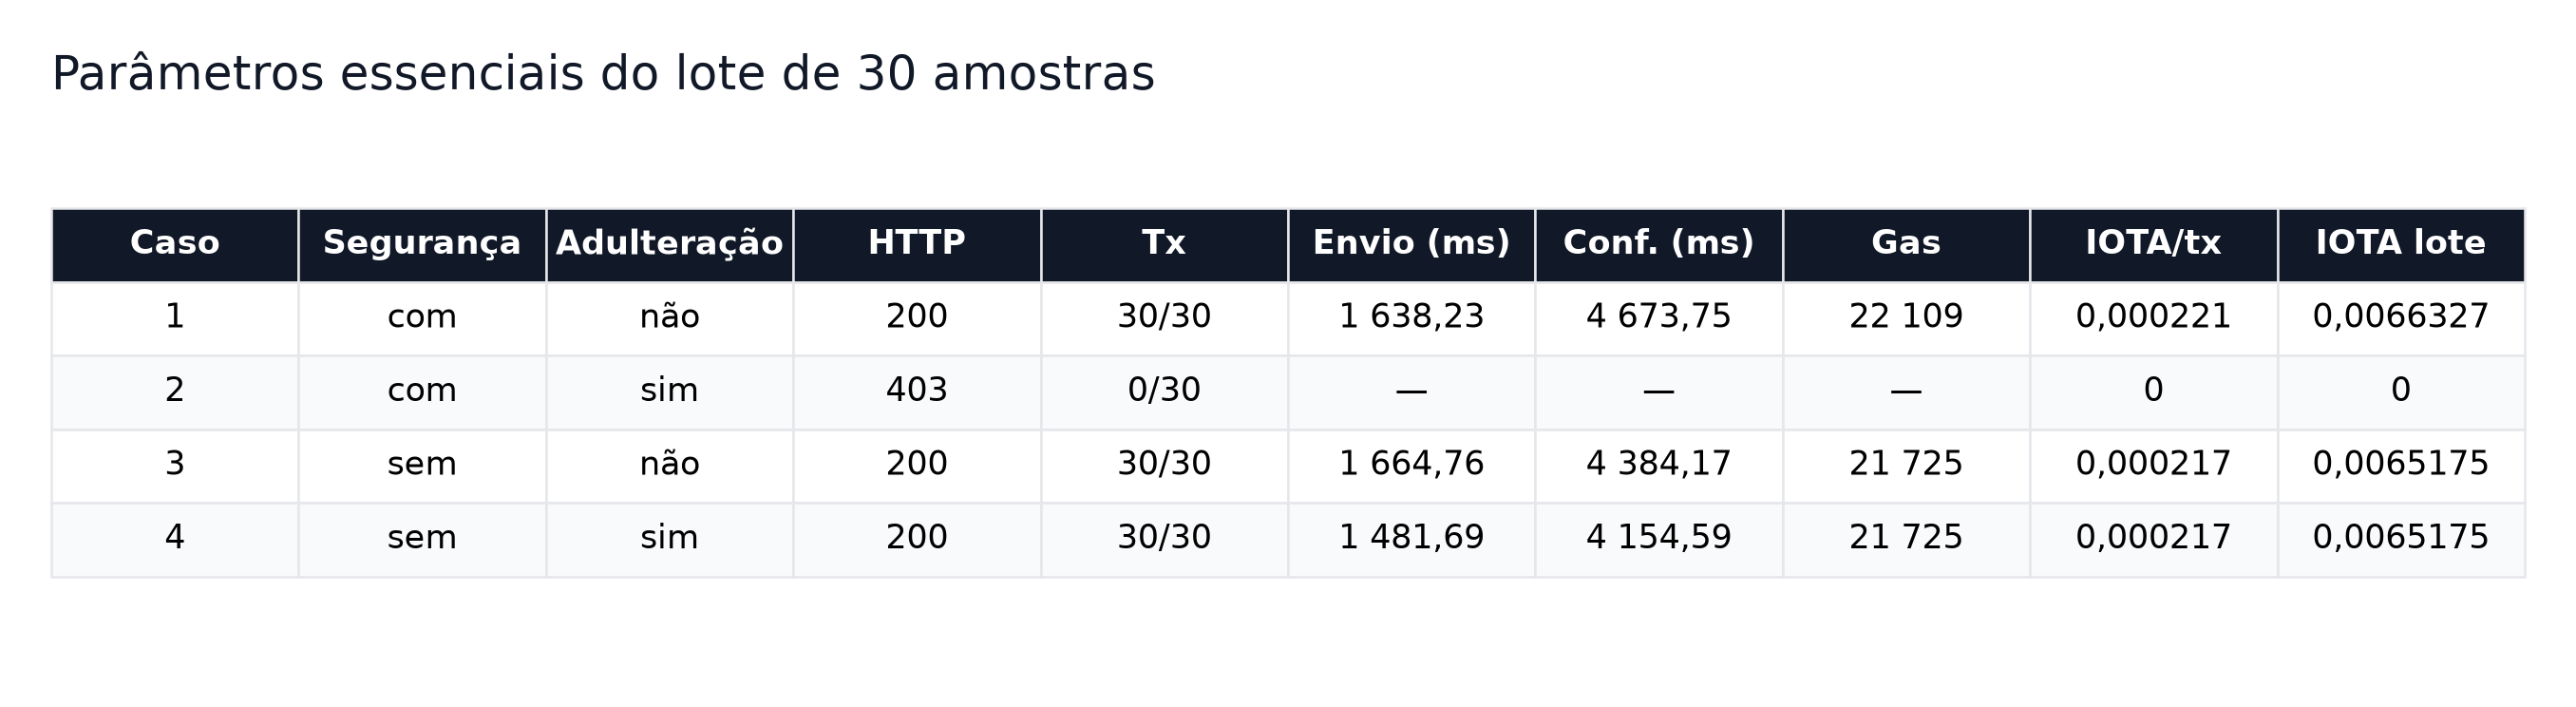
\includegraphics[width=\textwidth]{figuras/tabela-comparacao.png}
\caption{Parâmetros essenciais do lote (envio, confirmação, gás e custo). Caso~2 não gera transação.}
\label{fig:tabela-comparacao}
\end{figure}

\paragraph{Taxa de sucesso (lote sequencial, não carga).}
A Figura~\ref{fig:taxa-sucesso} mostra o fato: com allowlist, firmware limpo passa e firmware adulterado é recusado por completo; sem allowlist, firmware limpo e adulterado passam ambos. Isso não é throughput sob carga --- o intervalo entre envios foi sequencial.

\begin{figure}[htbp]
\centering
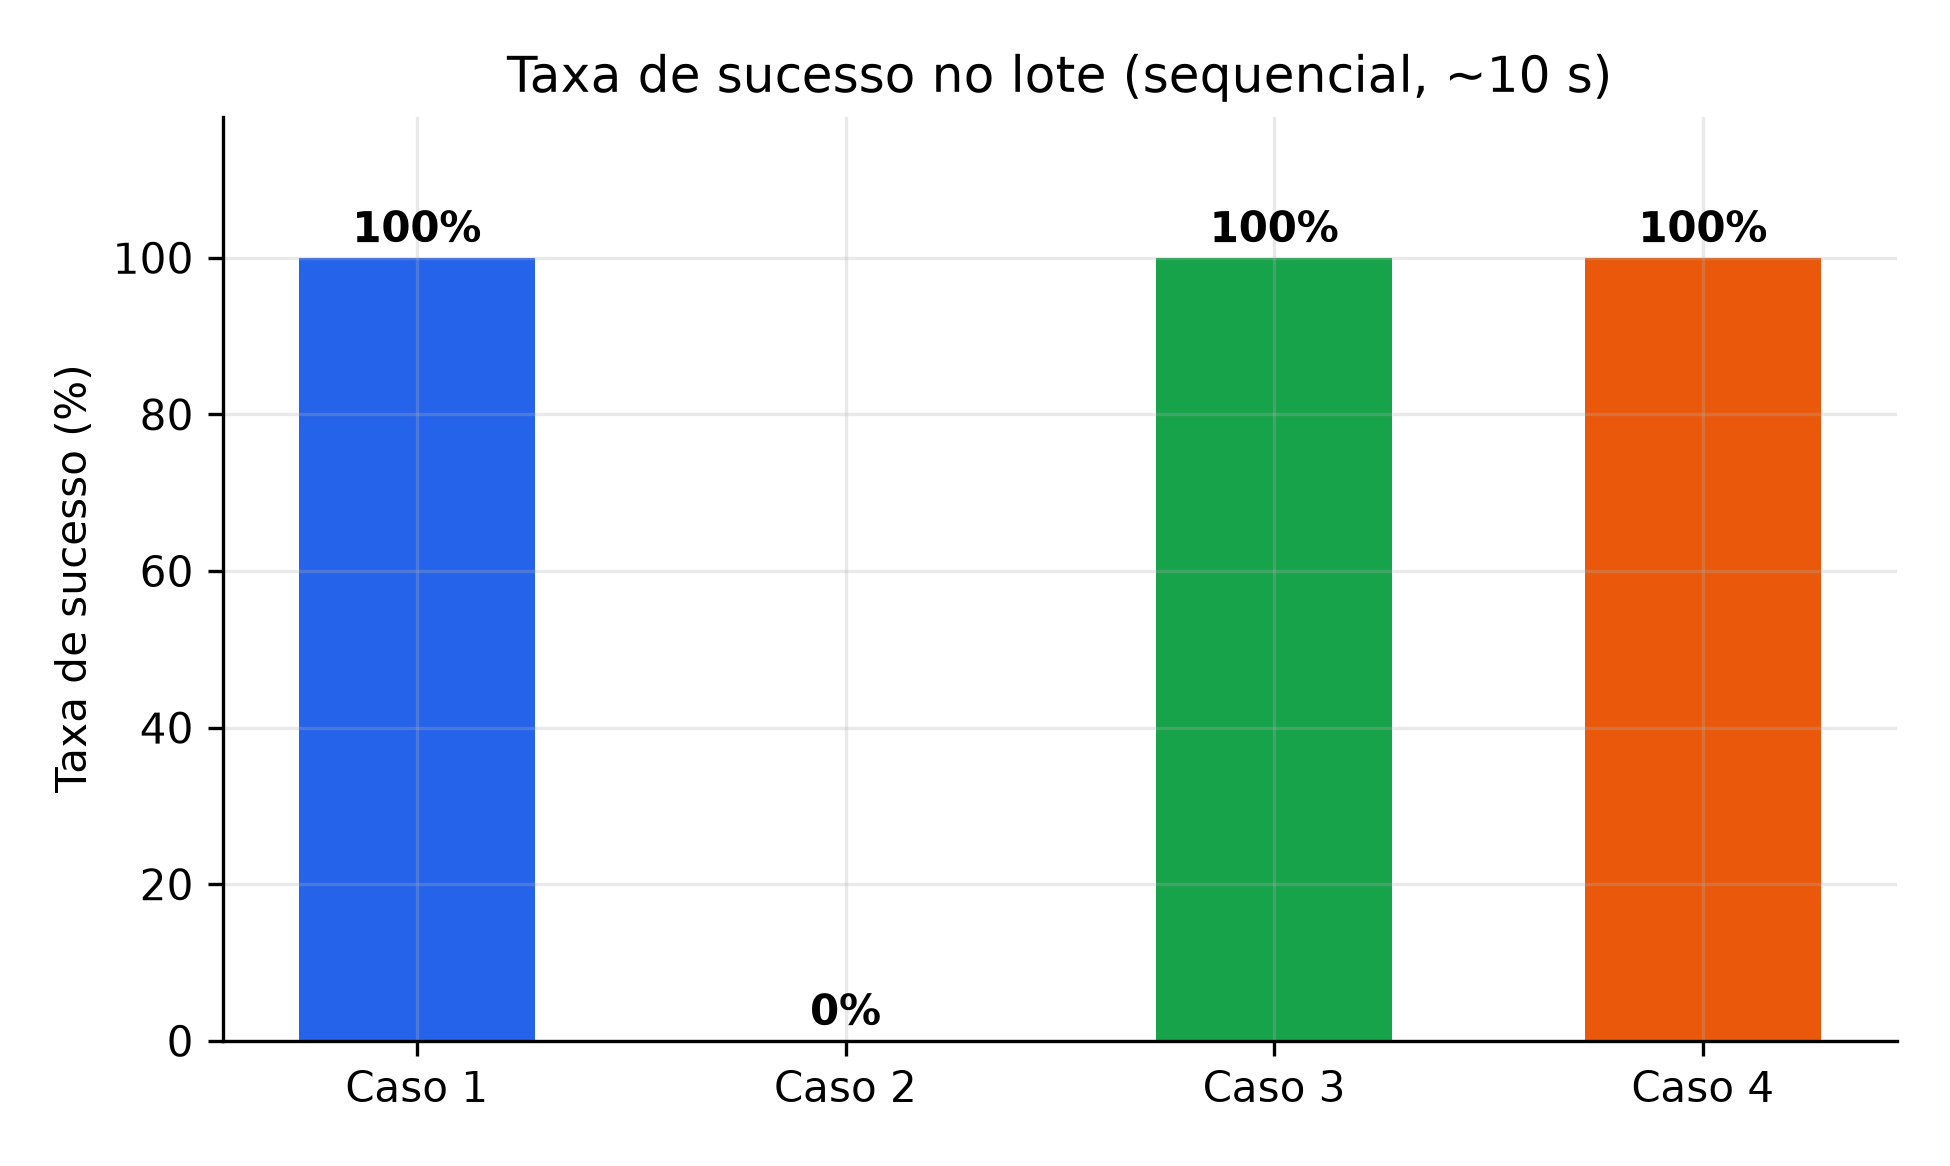
\includegraphics[width=0.78\textwidth]{figuras/taxa-sucesso.png}
\caption{Taxa de sucesso no lote. Com segurança: sucesso no firmware limpo e falha no adulterado. Sem segurança: sucesso nos dois.}
\label{fig:taxa-sucesso}
\end{figure}

\paragraph{Latência de confirmação.}
A Figura~\ref{fig:latencia-confirmacao} compara o tempo médio até a confirmação on-chain; a Figura~\ref{fig:serie-confirmacao} mostra a série amostra a amostra. O Caso~2 não aparece (HTTP 403, sem transação). A espera é a do bloco na testnet, não a da allowlist: os três caminhos com transação ficam na mesma ordem de grandeza, com desvio-padrão visível.

\begin{figure}[htbp]
\centering
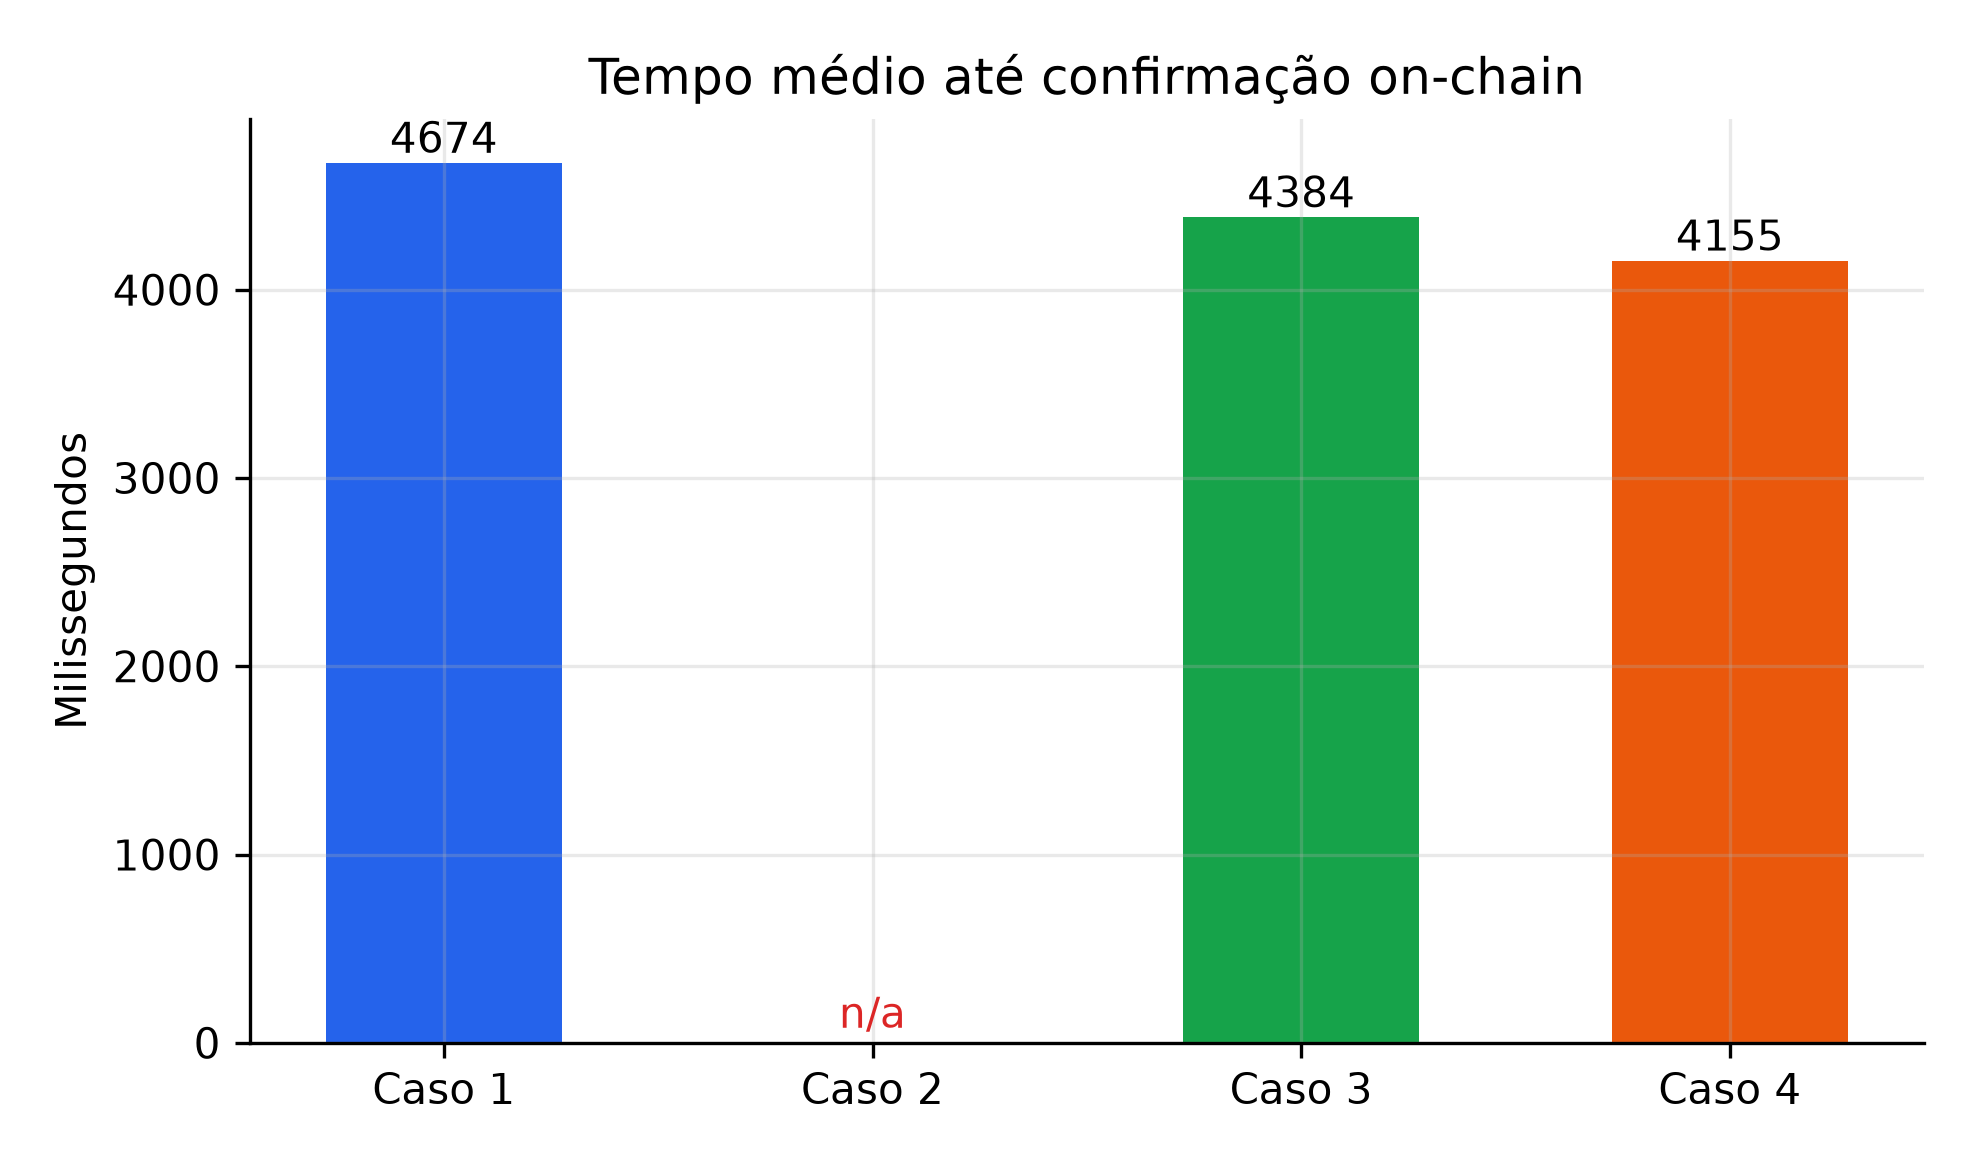
\includegraphics[width=0.78\textwidth]{figuras/latencia-confirmacao.png}
\caption{Tempo médio até a confirmação on-chain. Sem transação no tratamento com segurança e firmware adulterado.}
\label{fig:latencia-confirmacao}
\end{figure}

\begin{figure}[htbp]
\centering
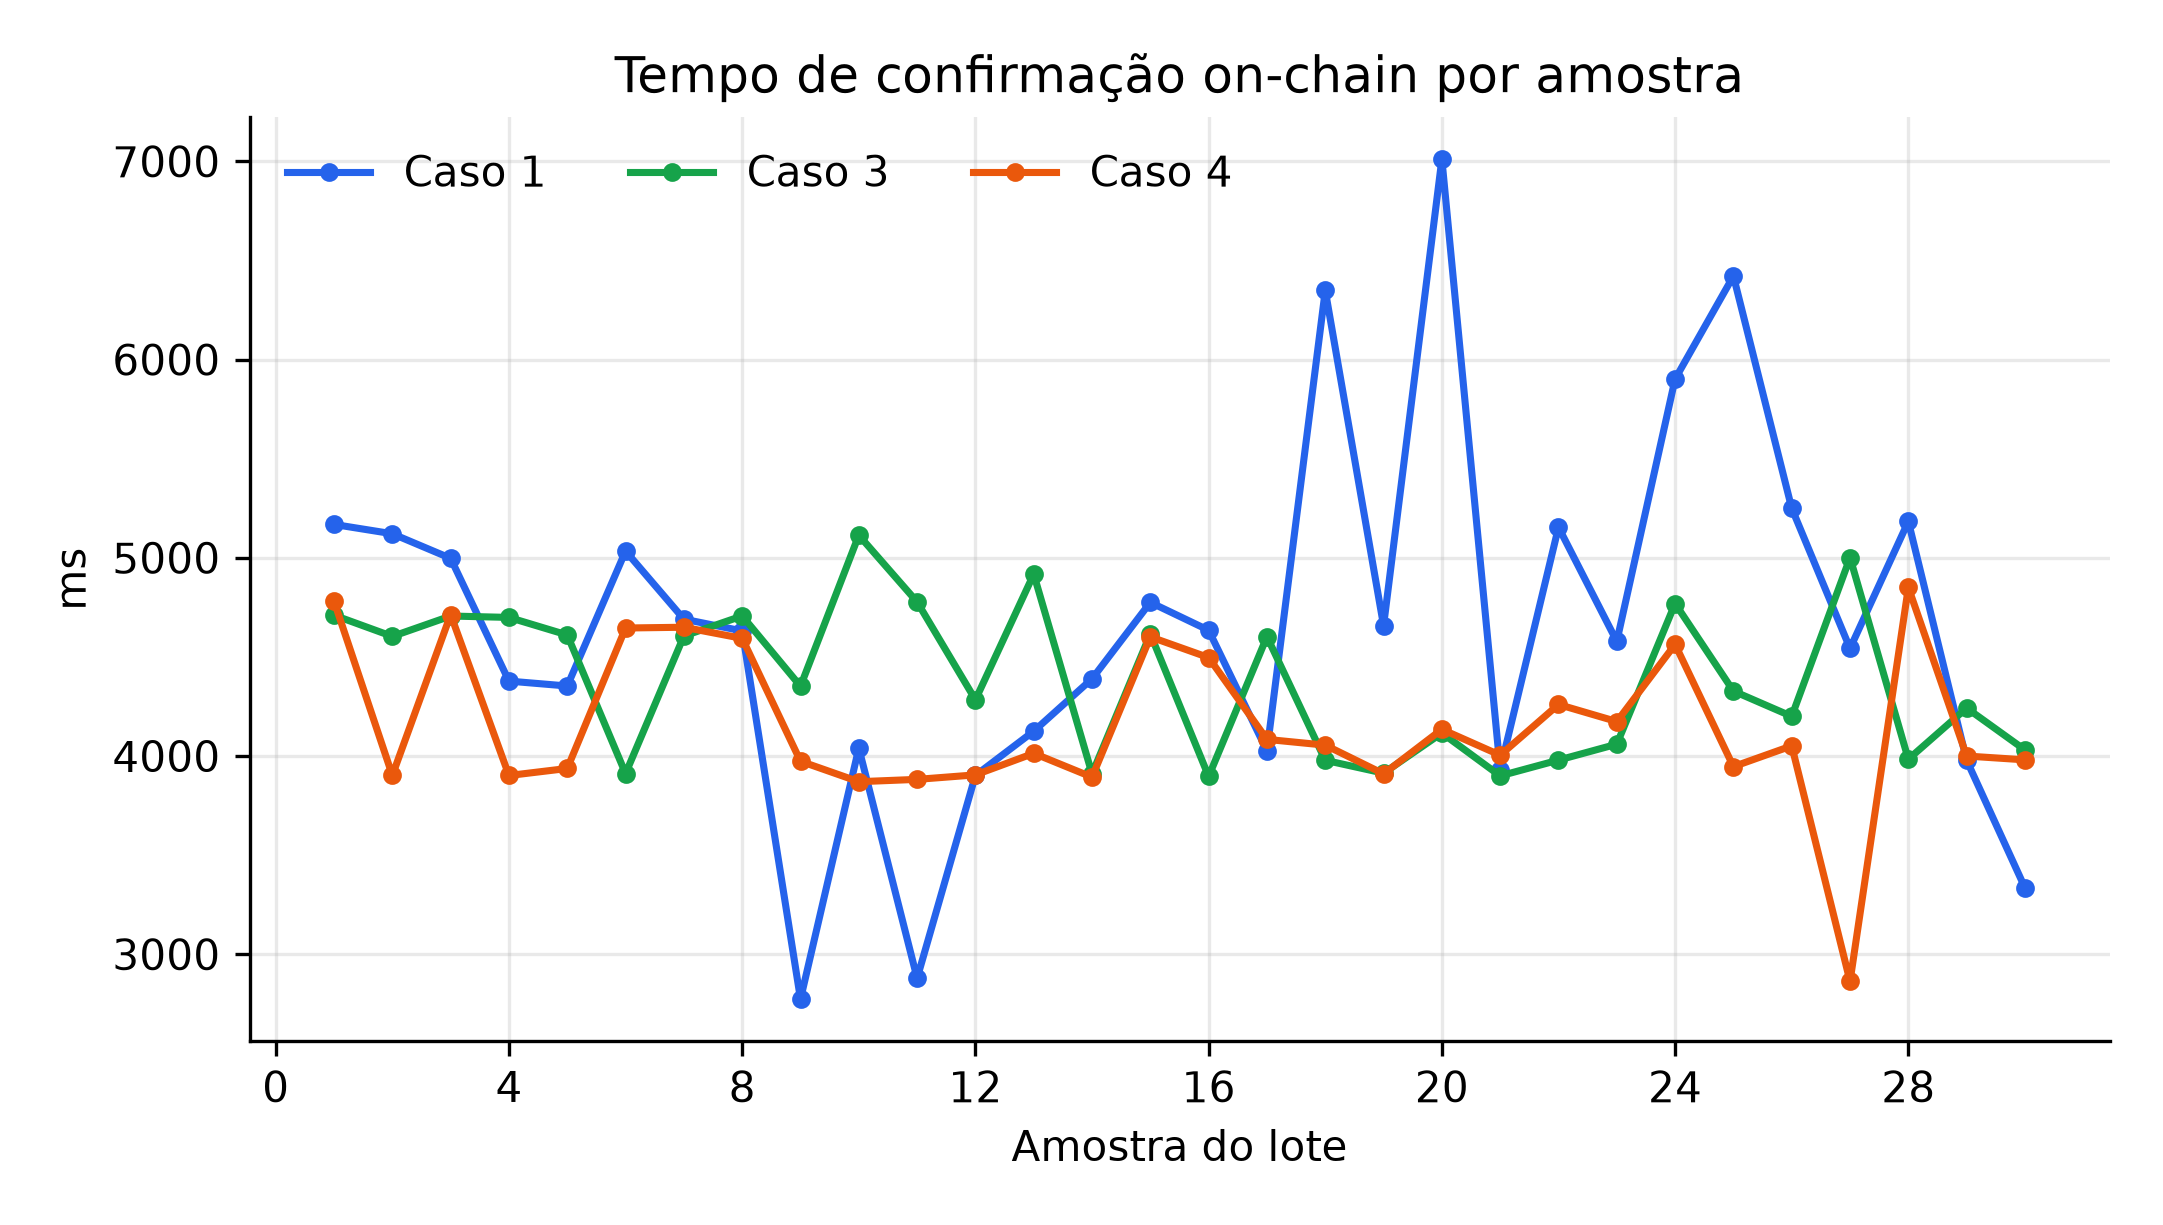
\includegraphics[width=0.92\textwidth]{figuras/serie-confirmacao.png}
\caption{Confirmação on-chain por amostra (somente tratamentos que geraram transação).}
\label{fig:serie-confirmacao}
\end{figure}

\paragraph{Custo em gás por atestação.}
A Figura~\ref{fig:custo-gas} mostra o gás médio por transação. Nos caminhos que gravaram na cadeia o gás foi constante em todas as amostras ($s=0$). A diferença entre com e sem allowlist é pequena porque os dois chamam o mesmo contrato \texttt{registrar}. Com segurança e firmware adulterado o custo é zero: o relay aborta antes da transação. O custo em IOTA (Figura~\ref{fig:custo}) segue o gás.

\begin{figure}[htbp]
\centering
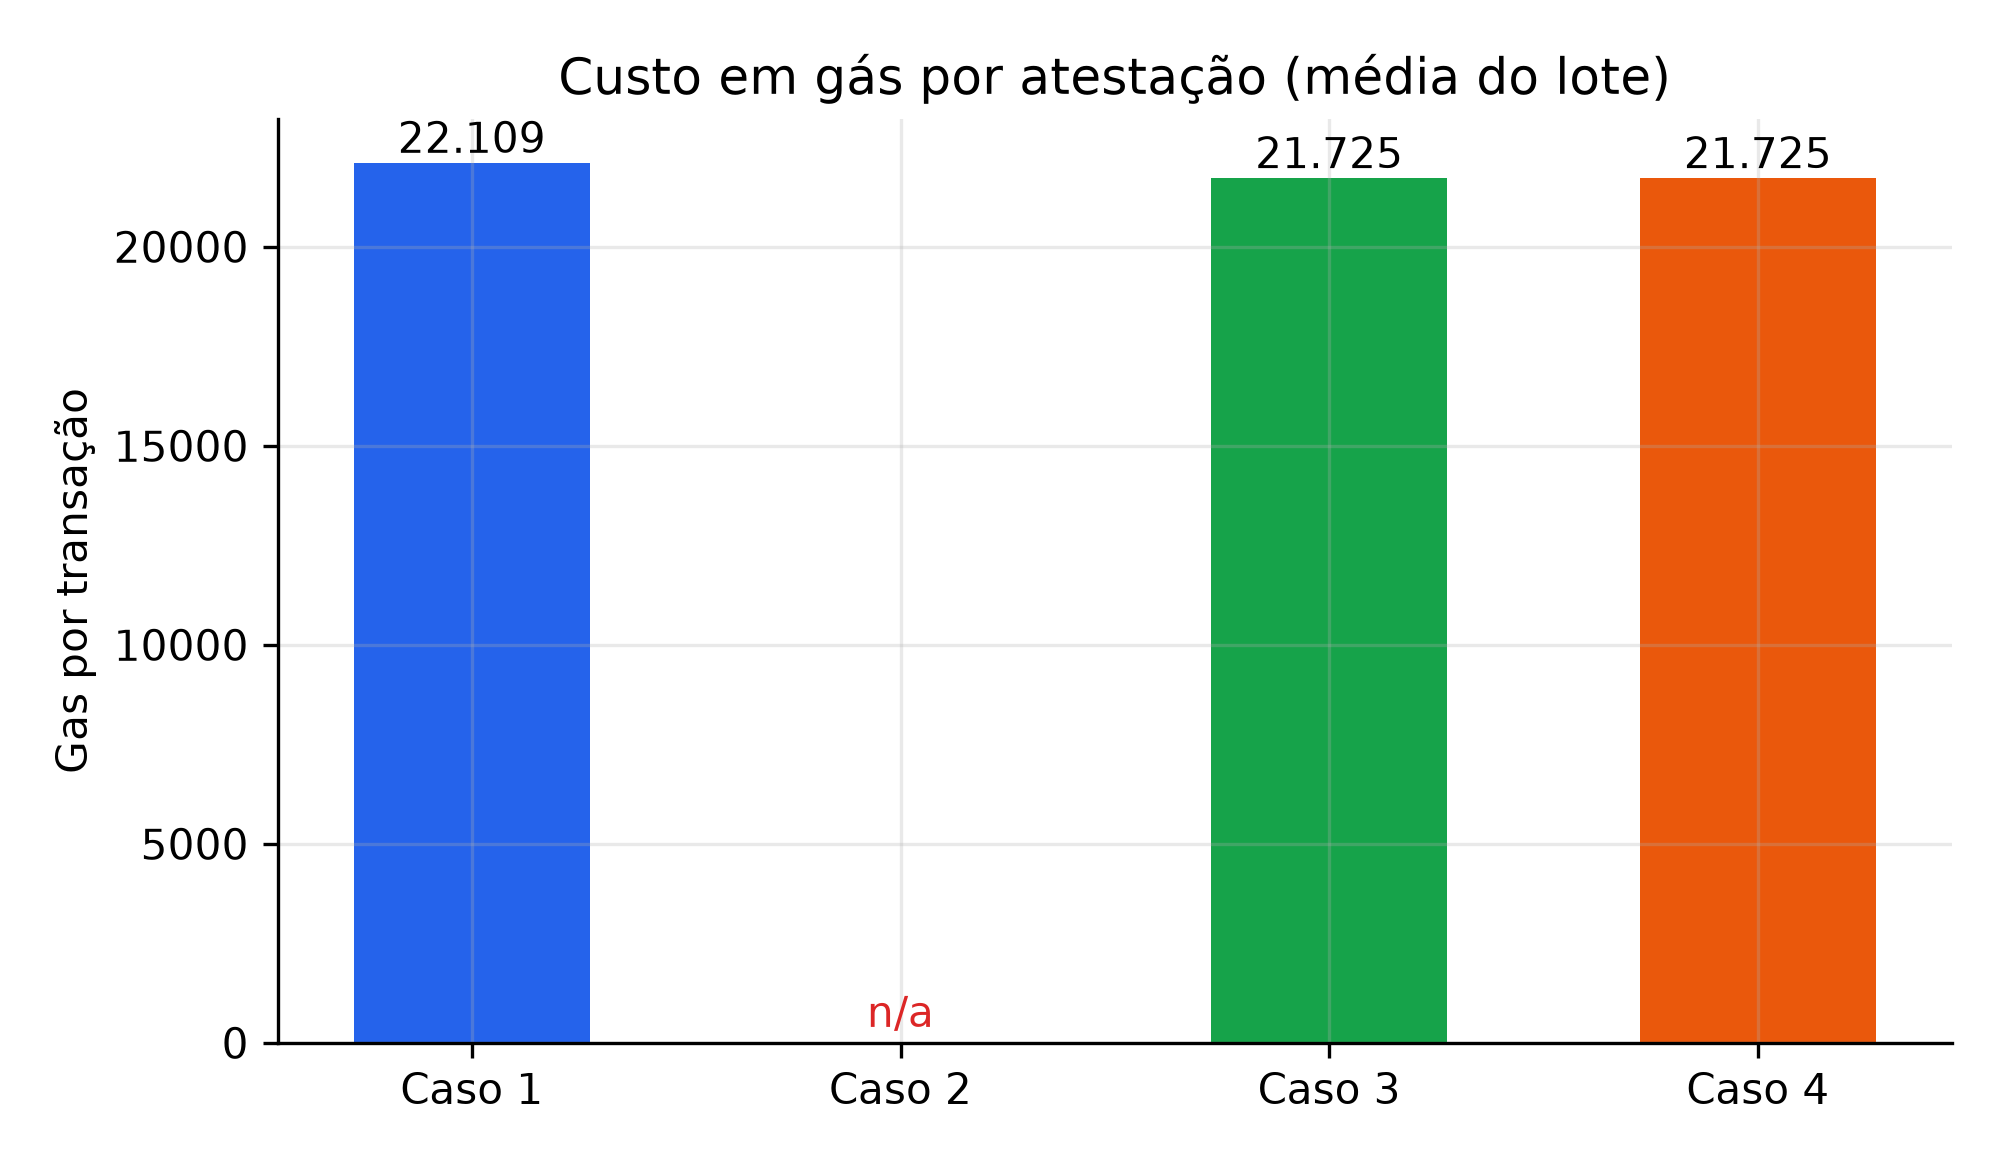
\includegraphics[width=0.78\textwidth]{figuras/custo-gas.png}
\caption{Gás médio por transação. Constante em cada caminho com transação; indefinido quando a allowlist recusa o hash.}
\label{fig:custo-gas}
\end{figure}

\begin{figure}[htbp]
\centering
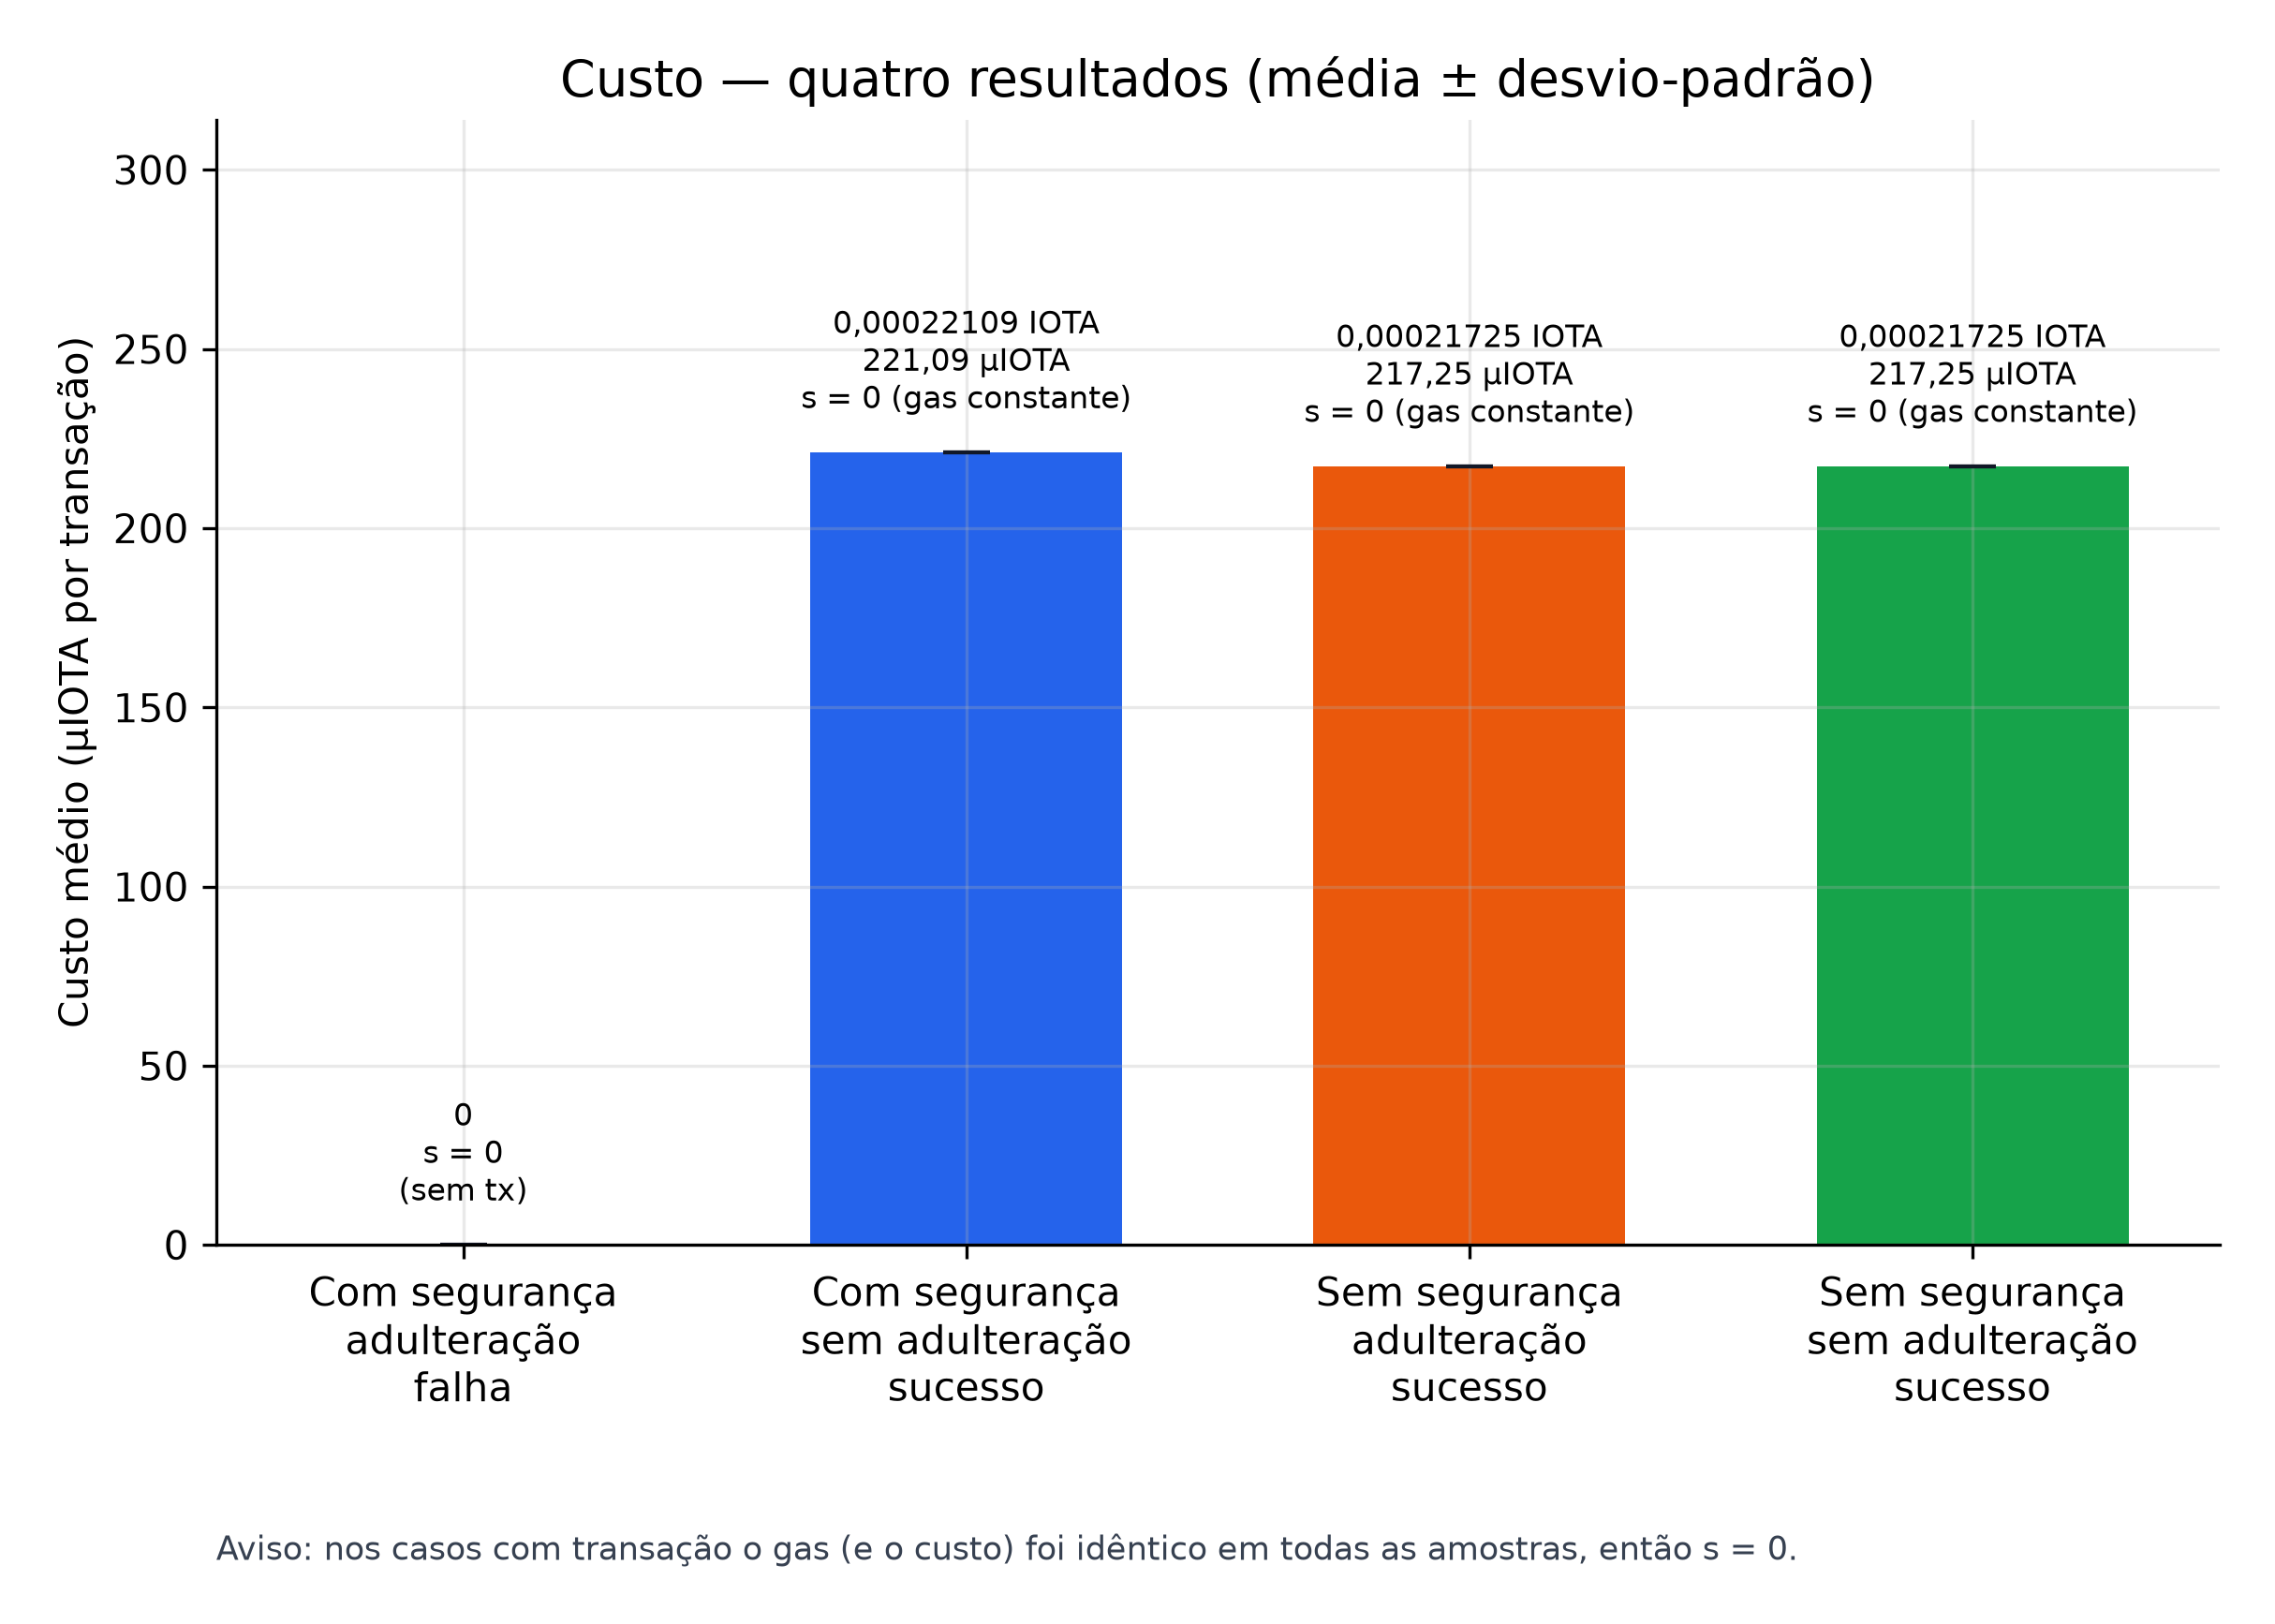
\includegraphics[width=0.92\textwidth]{figuras/custo.png}
\caption{Custo médio por transação nos quatro tratamentos. Gás constante ($s=0$) quando há transação; custo zero quando a allowlist recusa o hash.}
\label{fig:custo}
\end{figure}

\paragraph{Tempo de envio no relay (não é assinatura no ESP32).}
Não há figura de tempo de assinatura no chip: o ESP32 apenas faz POST HTTP; a carteira EVM assina no computador. A Figura~\ref{fig:tempo-envio-relay} e a Figura~\ref{fig:tempo} reportam o tempo até o relay enviar a transação e, ao lado, a confirmação. O overhead da allowlist nesse POST é pequeno neste lote.

\begin{figure}[htbp]
\centering
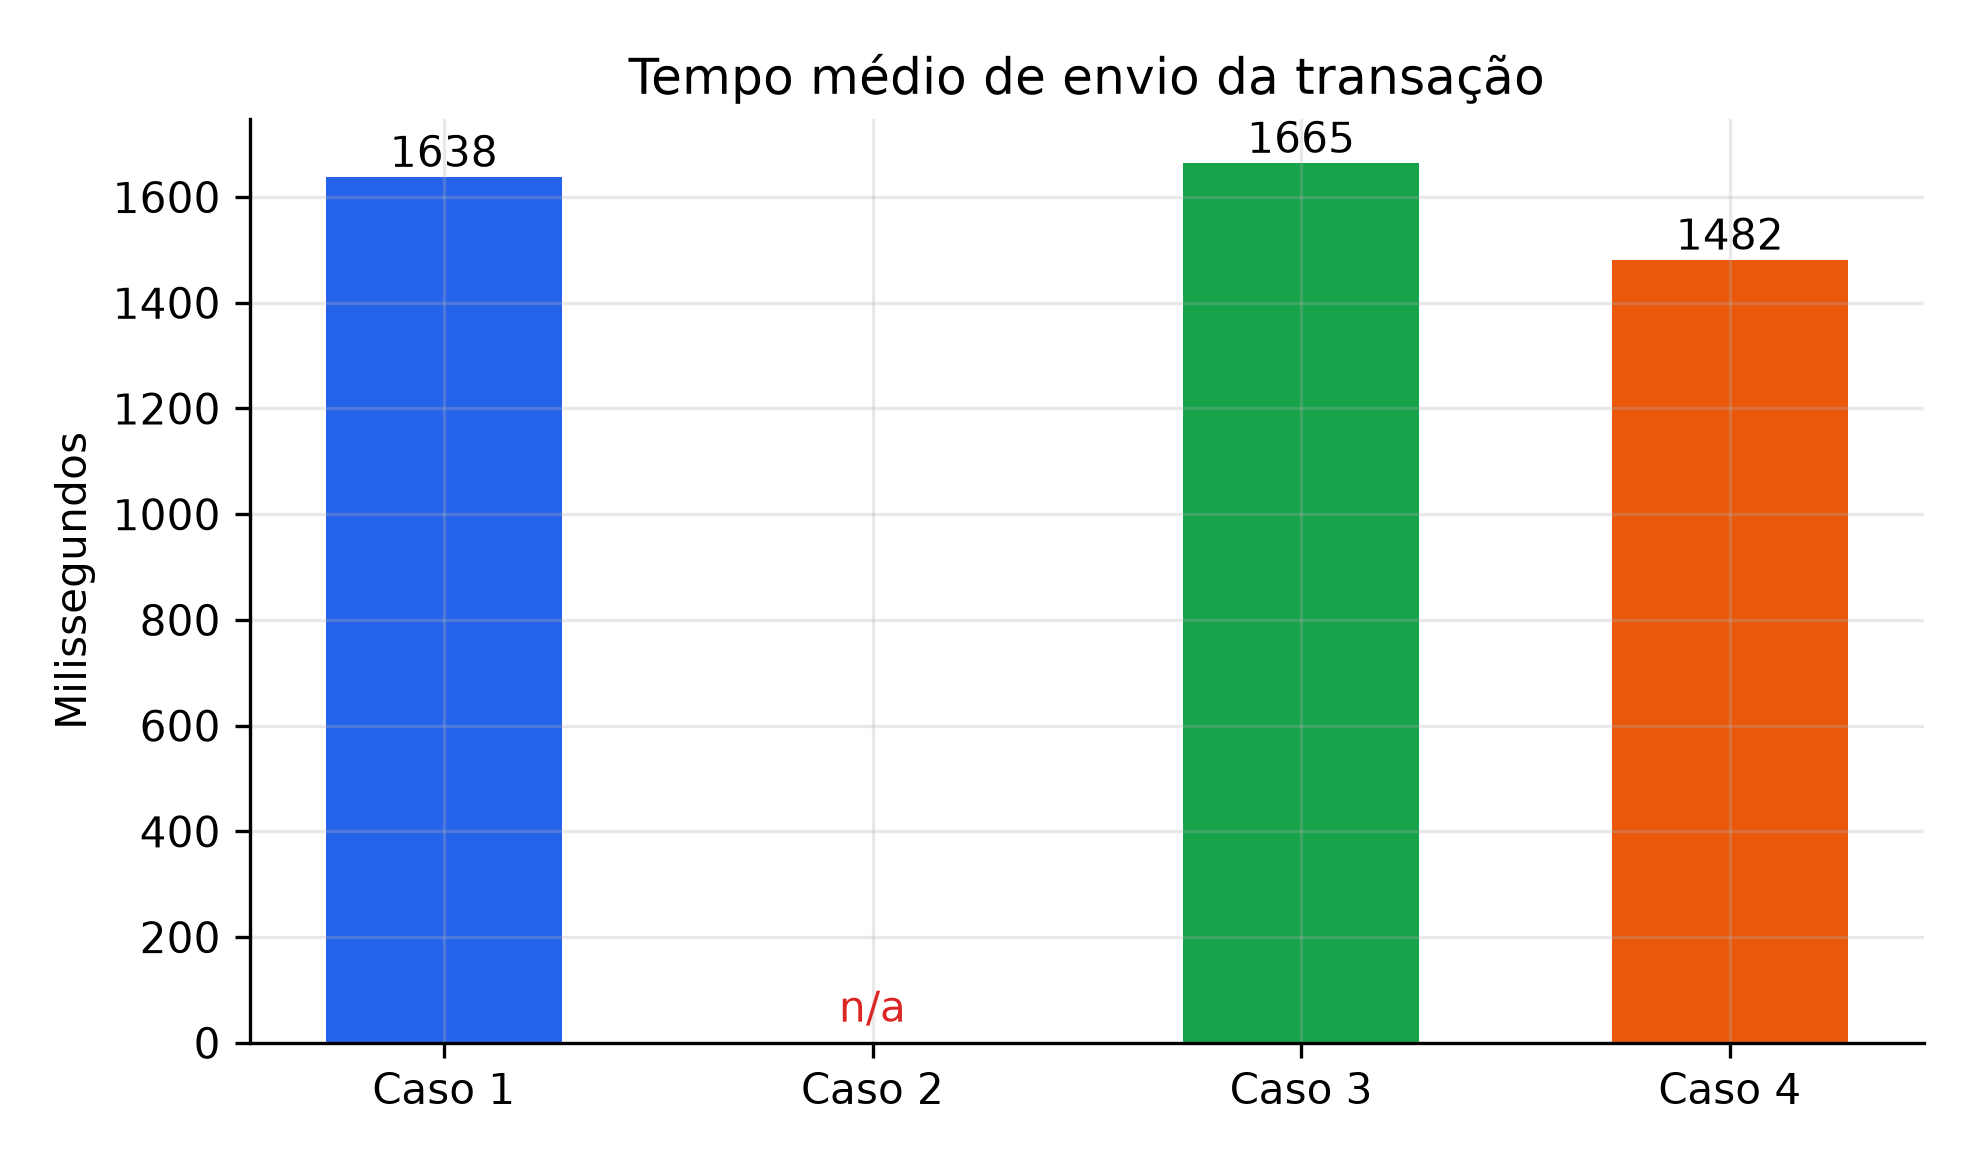
\includegraphics[width=0.78\textwidth]{figuras/tempo-envio-relay.png}
\caption{Tempo médio de envio da transação no relay. O tratamento com segurança e firmware adulterado não envia transação.}
\label{fig:tempo-envio-relay}
\end{figure}

\begin{figure}[htbp]
\centering
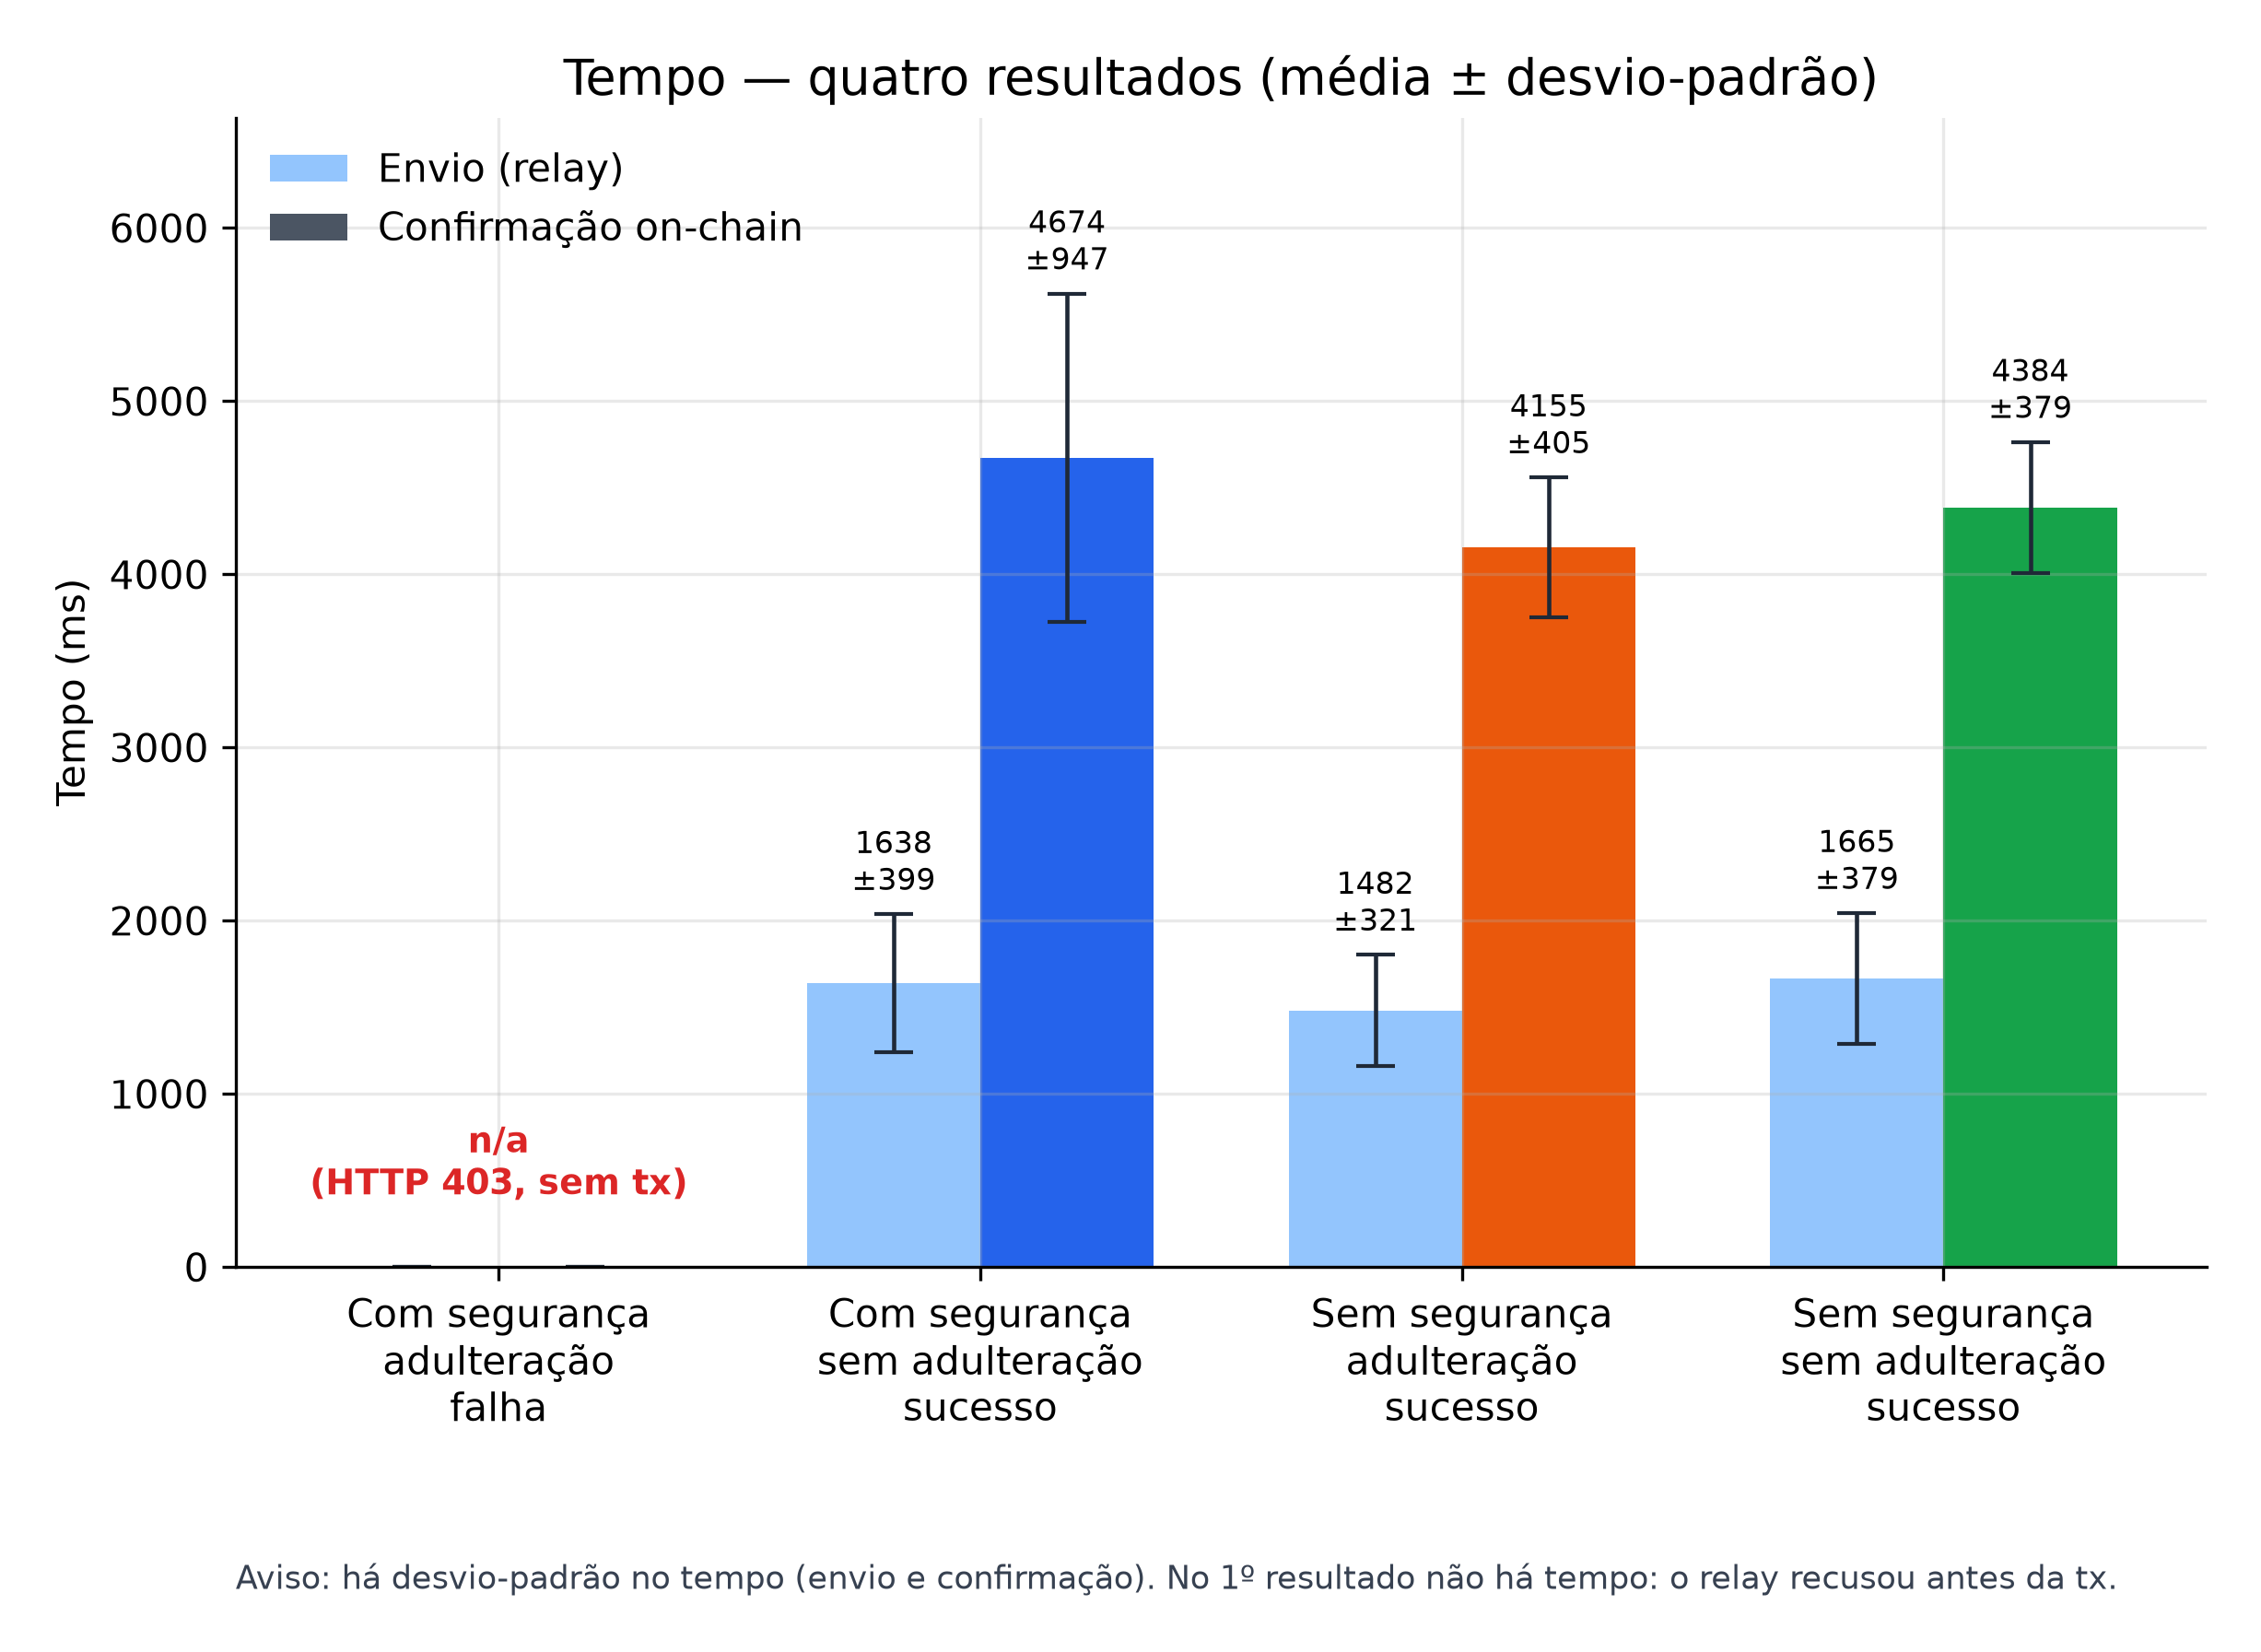
\includegraphics[width=0.92\textwidth]{figuras/tempo.png}
\caption{Envio e confirmação (média $\pm$ desvio-padrão) nos quatro tratamentos. Há desvio-padrão no tempo; o primeiro tratamento à esquerda não tem transação.}
\label{fig:tempo}
\end{figure}
